\documentclass[10pt]{article}
\usepackage[utf8]{inputenc}
\usepackage[T1]{fontenc}
\usepackage{amsmath}
\usepackage{amsfonts}
\usepackage{amssymb}
\usepackage[version=4]{mhchem}
\usepackage{stmaryrd}
\usepackage{graphicx}
\usepackage[export]{adjustbox}
\graphicspath{ {./images/} }

\title{SOLUTIONS FOR EXTRA ADMISSIONS TEST IN MATHEMATICS, COMPUTER SCIENCE AND JOINT SCHOOLS DECEMBER 2021 }

\author{}
\date{}


\begin{document}
\maketitle
A We can rewrite each of these to be $\cos (x)$ for some angle $x$ with $0<x<180^{\circ}$. Option (a) is $\cos \left(10^{\circ}\right)$. Option (b) is $\cos \left(25^{\circ}\right)$. Option (c) is $\cos \left(15^{\circ}\right)$. Option (d) is $\cos \left(5^{\circ}\right)$. Option (e) is $\cos \left(20^{\circ}\right)$. Now $\cos (x)$ is a decreasing function of $x$ between 0 and $180^{\circ}$, so the largest value is $\cos \left(5^{\circ}\right)$

The answer is (d)

B The first few terms of the binomial expansion of $\left(\left(x^{2}+x y\right)+y^{2}\right)^{n}$ are

$$
\left(\begin{array}{l}
n \\
0
\end{array}\right) y^{2 n}+\left(\begin{array}{l}
n \\
1
\end{array}\right)\left(x^{2}+x y\right) y^{2 n-2}+\left(\begin{array}{l}
n \\
2
\end{array}\right)\left(x^{2}+x y\right)^{2} y^{2 n-4}+\left(\begin{array}{l}
n \\
3
\end{array}\right)\left(x^{2}+x y\right)^{3} y^{2 n-6}+\ldots
$$

The first two terms don't contain any $x^{3} y^{2 n-3}$ terms, and any terms after these four must have a factor of $x^{4}$, so they don't contribute either. We need to think about the expansion of $\left(x^{2}+x y\right)^{2}$ which includes $2 x^{2} x y$, and the expansion of $\left(x^{2}+x y\right)^{3}$ which includes $(x y)^{3}$. So the coefficient is $2 \times\left(\begin{array}{l}n \\ 2\end{array}\right)+\left(\begin{array}{l}n \\ 3\end{array}\right)$.

The answer is (c)

C The quadrilateral looks like this

\begin{center}
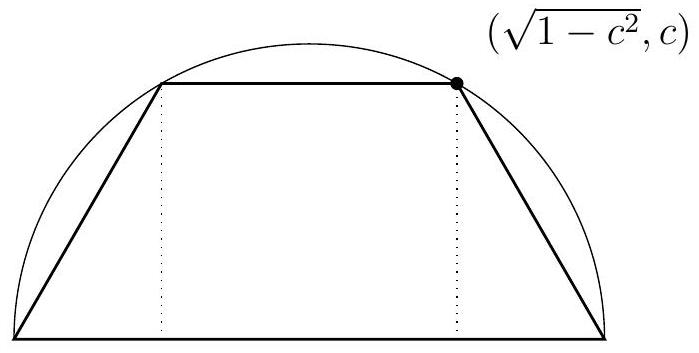
\includegraphics[max width=\textwidth]{2024_03_31_24d21beca0d7dc415c9ag-1}
\end{center}

The area is $c+c \sqrt{1-c^{2}}$. That's clearly bigger than $c$ since the second term is positive (this rules out options (a) and (e) and arguably (b)). Near to $c=1$, the second part of the function steeply decreases to zero, a bit like the corner of a semi-circle. The area is therefore larger than 1 for values of $c$ that are less than 1 but very near to 1 . That matches with graph option (d). The answer is (d)

D At time $t=1$ the particle reaches $x=1$. After a further 2 units of time the particle reaches $x=2$. This continues, and a geometric series shows that the particle reaches $x=n$ at time $t=2^{n}-1$. So the particle reaches $x=6$ at time $t=63$. Its speed immediately becomes $2^{-6}$ so it would take 64 further units of time to reach $x=7$. But just 37 units of time after the particle reached $x=6$, the time is $t=100$ and the particle is at $x=6+37 / 64=421 / 64$.

The answer is (d)

E The given polynomial is $\left(x^{2}-k\right)^{2}-(x-1)^{2}$ which can be factorised as

$$
\left(x^{2}-k-x+1\right)\left(x^{2}-k+x-1\right) \text {. }
$$

The first quadratic has two real roots if and only if $k>3 / 4$. The second quadratic has two real roots if and only if $k>-5 / 4$. So for four real roots we would need $k>3 / 4$. But we need\\
those four roots to be distinct, so we need to check that none of the roots of the first quadratic are also roots of the second quadratic. Equating the quadratics, this happens only if $x=1$, which is a root if and only if $k=1$. So we have exactly four real roots if $3 / 4<k<1$ or $k>1$ but for no other values of $k$.

\section*{The answer is (e)}
F The line $A B$ is a diameter, so the angle $A O B$ is a right angle. The line through $A$ and the origin is $y=4 x / 3$ and it must be perpendicular to the line through $B$ and the origin, so that line is $y=-3 x / 4$. Finally, the distance between $B$ and the origin is 10 , so we need to choose the two points on this line with the correct distance.

The answer is (d)

G The number 123, 456, 789 is a multiple of 3 because the sum of its digits is 45, which is a multiple of 3 . So its square is also a multiple of 3 . Check the sum of the digits of each of these numbers; reading from the front $1+5+2+4+1+5+7+8$ is a multiple of 3 , and reading from the other end $1+9+5+2+1$ is a multiple of 3 . So we need the remaining two digits ( 7 and the digit that's different in each option) to sum to a multiple of 3 . Only 5 does this.

The answer is (c)

H First try substituting in $x=1$ and $y=1$. This gives $2 f(1)=\frac{1}{f(1)}$ which we can solve for $f(1)= \pm \frac{1}{\sqrt{2}}$. The function is positive, so we take the positive root. Now set $y=1$ for $f(x)+\frac{1}{\sqrt{2}}=\frac{1}{f(x)}$ which is another quadratic, this time for $f(x)$. The positive solution is $f(x)=\frac{1}{\sqrt{2}}$. So the function is constant; it's $\frac{1}{\sqrt{2}}$ for all values of $x$, including $x=2021$.

The answer is $(\mathrm{d})$

I Write

$$
A=\int_{a}^{b} \log _{c} \sin ^{2} x \mathrm{~d} x, \quad B=\int_{a}^{b} \log _{c} \cos ^{2} x \mathrm{~d} x
$$

The given equations are $3 A-B=1$ and $A+B=3$ with solution $A=1, B=2$. The integral we're asked for is $2 A+B$ which is 4 .

The answer is (a)

$\mathbf{J}$ If the line is normal to the cubic in two places then the gradient of the cubic is equal at those two points. By symmetry of the derivative of the cubic, these points must be $\pm a$ for some real $a$. Then by rotational symmetry of the graph of the cubic, the normal line must go through the origin. So we must find values of $m$ such that $y=m x$ is normal to the given curve at some point.

The points of intersection are at $x= \pm \sqrt{k+m}$. The tangent should be normal to the line $y=m x$, so $\left(3 x^{2}-k\right) m=-1$ at either of those points of intersection. This simplifies to $(3 m+2 k) m=-1$. This is a quadratic with solutions if and only if $k^{2} \geq 3$. But we need to make sure that the points of intersection at $x= \pm \sqrt{k+m}$ actually exist.

The roots of the quadratic are $m=\frac{1}{3}\left(-k \pm \sqrt{k^{2}-3}\right)$. If $k>0$ then the larger root clearly gives $k+m>0$. However if $k<0$ then for $k+m>0$, we would need $2 k+\sqrt{k^{2}-3}>0$ which would imply that $4 k^{2}<k^{2}-3$, which is impossible. So only the case $k \geq \sqrt{3}$ gives a line that's normal to the cubic with a real point of intersection.

The answer is (a)


\end{document}